\documentclass{article}

\usepackage[breaklinks]{hyperref}
\usepackage[T1]{fontenc}
\usepackage[utf8]{inputenc}
\usepackage{graphicx}
\usepackage{lmodern}
\usepackage{mdframed}
\usepackage{amssymb,amsfonts,amsmath,amsthm}
\usepackage{mathtools}
\usepackage{bm}
\usepackage{listings}
\usepackage{enumerate}
\usepackage{float}
\usepackage{fullpage}
\usepackage{xcolor}
\usepackage{tikz}
\usepackage{pgfplots}
\usepackage{pgf}
\usepackage{tikz}
\usetikzlibrary{arrows,automata}
%\usepgfplotslibrary{colormaps}

\definecolor{RED}{HTML}{EB6231}
\definecolor{YELLOW}{HTML}{E29D26}
\definecolor{BLUE}{HTML}{5D80B4}
\definecolor{LIGHTGREEN}{HTML}{6ABD9B}
\definecolor{GREEN}{HTML}{8FB03E}
\definecolor{PURPLE}{HTML}{BE1E2D}
\definecolor{BROWN}{HTML}{A97C50}
\definecolor{PINK}{HTML}{DA1C5C}

\pgfplotsset{every axis/.append style={line width=1pt}}
\pgfplotscreateplotcyclelist{colors}{RED\\YELLOW\\BLUE\\LIGHTGREEN\\GREEN\\}

\newcommand{\der}{\mathrm{d}}
\newcommand{\e}{\mathrm{e}}
\newcommand{\dnds}{dNdS}

% Time, effective population size and mutation rate.
\newcommand{\Ne}{N_\e}

% DNA
\newcommand{\SetNuc}{\Omega_{\mathrm{N}}}
\newcommand{\mutmatrix}{R}
\newcommand{\Mutmatrix}{\bm{\mutmatrix}}
\newcommand{\exchan}{\rho}
\newcommand{\Exchan}{\bm{\exchan}}
\newcommand{\mutequi}{\pi}
\newcommand{\Mutequi}{\bm{\mutequi}}

% Codons
\newcommand{\SetCodon}{\Omega_{\mathrm{C}}}
\newcommand{\ci}{{\color{RED}{i}}}
\newcommand{\cj}{{\color{GREEN}{j}}}
\newcommand{\itoj}{\ci, \cj}
\newcommand{\nucitoj}{\mathcal{M}(\itoj)}
\newcommand{\submatrix}{Q}
\newcommand{\Submatrix}{\bm{\submatrix}}
\newcommand{\subequi}{\Pi}
\newcommand{\Subequi}{\bm{\subequi}}
\newcommand{\probmatrix}{P}
\newcommand{\Probmatrix}{\bm{\probmatrix}}

% Amino-acids
\newcommand{\SetAa}{\Omega_{\mathrm{A}}}
\newcommand{\aminoacid}{\text{A}}
\newcommand{\aai}{\mathcal{A}(\ci)}
\newcommand{\aaj}{\mathcal{A}(\cj)}
\newcommand{\Ni}{\mathcal{V}\left(\ci\right)}
\newcommand{\NiNonSyn}{\mathcal{N}_{\mathrm{onSyn}}\left(\ci\right)}
\newcommand{\NiSyn}{\mathcal{S}_{\mathrm{yn}}\left(\ci\right)}
\newcommand{\fit}{f}
\newcommand{\Fit}{\bm{\fit}}
\newcommand{\fiti}{\fit_{\aai}}
\newcommand{\fitj}{\fit_{\aaj}}
\newcommand{\scaledfit}{F}
\newcommand{\ScaledFit}{\bm{\scaledfit}}
\newcommand{\scaledfiti}{\scaledfit_{\aai}}
\newcommand{\scaledfitj}{\scaledfit_{\aaj}}
\newcommand{\selcoef}{{\delta_{\fit}}}
\newcommand{\scaledselcoef}{{\Delta \scaledfit}}

% Tree
\newcommand{\Tree}{\mathcal{T}}
\newcommand{\taxon}{\text{m}}
\newcommand{\Ntaxa}{\text{N}_{\taxon}}
\newcommand{\branch}{\text{w}}
\newcommand{\branchexp}{^{(\branch)}}
\newcommand{\Nbranch}{\text{N}_{\branch}}
\newcommand{\up}{\branch^{\uparrow}}
\newcommand{\down}{\branch_{\downarrow}}
\newcommand{\node}{\text{v}}
\newcommand{\nodeexp}{^{(\node)}}
\newcommand{\Nnode}{\text{N}_{\node}}
\newcommand{\age}{T}
\newcommand{\branchtime}{\Delta \age}
\newcommand{\branchlength}{L}

% Alignment
\newcommand{\site}{\text{s}}
\newcommand{\siteexp}{^{(\site)}}
\newcommand{\Nsite}{\text{N}_{\site}}
\newcommand{\branchsiteexp}{^{(\branch, \site)}}
\newcommand{\rootsiteexp}{^{(\text{Root}, \site)}}
\newcommand{\Data}{{\color{PINK}{D}^{k}}}
\newcommand{\sn}{{\color{BLUE}{S}}}
\newcommand{\s}{{\color{LIGHTGREEN}{S_0^{k}}}}
\newcommand{\si}{{\color{PINK}{S_1^{k}}}}
\newcommand{\sii}{{\color{PINK}{S_2^{k}}}}
\newcommand{\siii}{{\color{PINK}{S_3^{k}}}}
\newcommand{\siiii}{{\color{PINK}{S_4^{k}}}}
\newcommand{\siiiii}{{\color{LIGHTGREEN}{S_5^{k}}}}

% Categories
\newcommand{\cat}{\text{k}}
\newcommand{\catvar}{K}
\newcommand{\catexp}{^{(\cat)}}
\newcommand{\Ncat}{\text{N}_{\cat}}
\newcommand{\catsite}{\mathcal{K}\left(\site\right)}
\newcommand{\catsiteexp}{^{(\catsite)}}
\newcommand{\branchcatexp}{^{(\branch, \cat)}}
\newcommand{\rootcatexp}{^{(\text{Root}, \cat)}}

% Polymorphism
\newcommand{\copies}{\text{n}}
\newcommand{\samples}{\text{N}_{\copies}}

% Random variables
\newcommand{\uniform}{\bm{U}}
\newcommand{\brownian}{\bm{B}}
\newcommand{\contrast}{\bm{C}}
\newcommand{\covariance}{\bm{\Sigma}}
\newcommand{\covariancedf}{q}
\newcommand{\covariancekappa}{\kappa}
\newcommand{\base}{D}
\newcommand{\Base}{\bm{\base}}
\newcommand{\baseconc}{\alpha}
\newcommand{\Basecenter}{\gamma}
\newcommand{\stickbreaking}{\omega}
\newcommand{\StickBreaking}{\bm{\stickbreaking}}
\newcommand{\stickbreakinghyper}{\beta}

% Mapping
\newcommand{\history}{\mathcal{H}}

\author{Thibault Latrille.}
\title{Inferring ancient demographic history \\with Mutation-Selection models.}

\begin{document}

\maketitle
\section*{Abstract}

Selection in protein-coding sequences can be detected based on multiple sequence alignments using phylogenetic codon models.
Mechanistic approaches, grounded on population-genetics first principles, have been recently developed.
These so-called mutation-selection models explicitly formalize the interplay between mutation, selection and drift, and return an estimate of the amino-acid fitness landscape, considered static along the phylogeny.
They were recently proposed as a null (nearly-neutral) model against which to test for the presence of adaptation (Rodrigue, Lartillot MBE 2016, Bloom, 2016).
However, these models rely on the assumption of multiplicative fitness landscapes (no epistasis) and constant population size; they also ignore polymorphism in extant species, with only one sequence representing the whole population.
As a result, they return potentially biased estimates.\\
	
We propose an extended mutation-selection model relaxing some of these assumptions, by accommodating for fluctuating population size and fluctuating mutation rate along the phylogeny, and by modeling polymorphism in extant species.
The resulting mechanistic framework allows for a reconstruction of long-term trends in population size along the phylogeny.
Simultaneously, it offers a better background for detecting adaptation across large clades, by correcting for local changes in the relative strength of selection and random drift.
Finally, our work also points to important theoretical questions about how coding sequences respond to changes in effective population size and to selection.

\newpage
\tableofcontents
\newpage

\section{Notations}

\subsection{Time, effective population size and mutation rate.}
\begin{itemize}
	\setlength\itemsep{-0.25em}
	\item $\Ne \in \mathbb{N}$ is the effective population size.
	\item $t \in \mathbb{R}_{\geq 0}$ is the time measured in unit of population size ($t=1 \Rightarrow 4 \Ne $ generations).
	\item $\mu \in \mathbb{R}_{\geq 0}$ is the DNA mutation rate for one site of the sequence per unit of time.
	\item $u \in \mathbb{R}_{\geq 0}$ is the DNA mutation rate for one site of the sequence per generation.
	\item $\tau = u / \mu \in \mathbb{R}_{\geq 0}$ is time per generation.
	\item $\theta=4 \Ne u \in \mathbb{R}_{>0} $ is the scaled mutation rate.
\end{itemize}

\subsection{DNA}
\begin{itemize}
	\setlength\itemsep{-0.25em}
	\item $ \SetNuc =\left\{ A,C,G,T \right\} $ is the set of $4$ nucleotides in lexicographic order.
	\item $a \in \SetNuc $ and $b \in \SetNuc $ are used to denote nucleotides.
	\item $\mutmatrix_{a,b} \in \mathbb{R}_{> 0}$ is the mutation rate from nucleotide $a$ to $b$.
	\item $\Mutmatrix \in \mathbb{R}_{> 0}^{4 \times 4} $ is the mutation rate matrix between nucleotides.
	\item $\Mutequi = \left(\mutequi_A , \mutequi_C , \mutequi_G , \mutequi_T \right) \in \left]0,1\right[^4$ is the vector of nucleotides stationary distribution.
\end{itemize}

\subsection{Codons}
\begin{itemize}
	\setlength\itemsep{-0.25em}
	\item $\SetCodon = \left\{ AAA,AAC, \dots, TTT \right\} $ is the set of $61$ non-stop codons in lexicographic order.
	\\By definition $\SetCodon = \SetNuc^3 \setminus \left\{ TAA, TAG, TGA \right\} $.
	\item $\ci \in \SetCodon $, and $\cj \in \SetCodon $ are used to denote the codons.
	\item $\ci = \left\{ \ci_1, \ci_2, \ci_3 \right\} $ is used to denote the nucleotides at first, second and third positions of the codon.
	\item $\Ni \subset \SetCodon $ is the set of neighboring codons of $\ci$ such that the codons are only one mutation away from $\ci$.
	\item $ \nucitoj \in \SetNuc^2 $ is the origin and target nucleotides 
	that changed if $\cj \in \Ni$.
	\item $\submatrix_{\itoj} \in \mathbb{R}_{\geq 0} $ is the substitution rate from codon $i$ to $j$.
	\item $\Submatrix \in \mathbb{R}_{\geq 0}^{61 \times 61} $ is the substitution rate matrix.
	\item $\Subequi = \left( \subequi_{\ci}, \ \forall \ci \in \SetCodon \right) \in \left]0,1\right[^{61} $ is the vector of codon stationary distribution.
\end{itemize}

\subsection{Amino-acids}
\begin{itemize}
	\setlength\itemsep{-0.25em}
	\item $\SetAa = \left\{ \mathrm{Arginine}, \dots ,\mathrm{Tyrosine} \right\} $ is the set of 20 amino-acids in lexicographic order.
	\item $\aai \in \SetAa $ and $\aaj \in \SetAa$ are used to denote the amino-acid encoded by codon $\ci$ and $\cj$.
	\item $\NiNonSyn = \left\{ \cj \in \Ni  \mid \aai \neq \aaj  \right\} \subset \Ni $ is the set of non-synonymous neighboring codons of codon $\ci$.
	\item $\NiSyn = \left\{ \cj \in \Ni  \mid \aai = \aaj  \right\} \subset \Ni $ is the set of synonymous neighboring codons of codon $\ci$.
	\item $\fit_{\aminoacid} \in \mathbb{R} $ is the fitness of amino-acid $\aminoacid$.
	\item $\Fit = \left( \fit_{\aminoacid}, \ \forall \aminoacid \in \SetAa \right) \in \mathbb{R}^{20} $ is the vector of amino-acids fitnesses.
	\item $\scaledfit_{\aminoacid} = 4 \Ne \fit_{\aminoacid} \in \mathbb{R} $ is the scaled fitness of amino-acid $\aminoacid$.
	\item $\ScaledFit = \left( \scaledfit_{\aminoacid}, \ \forall \aminoacid \in \SetAa \right) \in \mathbb{R}^{20} $ is the vector of amino-acids scaled fitnesses.
\end{itemize}

\subsection{Tree}
\begin{itemize}
	\setlength\itemsep{-0.25em}
	\item $\Tree$ is the rooted phylogenetic binary tree topology considered fixed.
	\item $\Ntaxa \in \mathbb{N}$ is the number of taxa for which we have a sequence.
	\item $\taxon \in \left\{ \taxon \in \mathbb{N} \mid 1 \leq \taxon \leq \Ntaxa \right\}$ is the $\taxon^{\mathrm{th}}$ taxon.
	\item $\Nbranch = 2 \Ntaxa - 2 \in \mathbb{N}$ is the number of branches of the tree.
	\item $\branch \in \left\{ \branch \in \mathbb{N} \mid 1 \leq \branch \leq \Nbranch \right\}$ is the $\branch^{\mathrm{th}}$ branch of the tree.
	\item $\Nnode = 2 \Ntaxa - 1 \in \mathbb{N}$ is the number of nodes of the tree.
	\item $\node \in \left\{ \node \in \mathbb{N} \mid 1 \leq \node \leq \Nnode \right\}$ is the $\node^{\mathrm{th}}$ node of the tree.
	\item $\up$ is the upper node of branch $\branch$, meaning the node closest to the root. Each branch has a different upper node, except for the branches attached to root which share the same upper node (the root).
	\item $\down$ is the lower node of branch $\branch$, meaning the node closest to the leaves supporting the branch. Each branch has a different lower node, and for the extant species the lower node is the leaf.
\end{itemize}

\subsection{Alignment}
\begin{itemize}
	\setlength\itemsep{-0.25em}
	\item $\Nsite \in \mathbb{N}$ is the number of codon sites in the sequence.
	\item $\site \in \left\{ \site \in \mathbb{N} \mid 1 \leq \site \leq \Nsite \right\}$ is the $\site^{\mathrm{th}}$ codon site of the sequence.
	\item $\catsite$ fitness category of site $\site$.
\end{itemize}

\newpage

\section{Evolution of protein-coding sequences}

Phylogenetic reconstruction seeks to infer past evolutionary history of life on Earth.
However, phylogeneticists are constrained to solely access present-day populations and extinct fossils.
One approach to circumvent this limitation is to study the evolution of molecular sequences backward in time, based on present day molecular sequences.
In this molecular framework, evolution is generally seen as a stochastic process, and the interplay between point mutations and the selection of these mutations leads to substitutions in sequences over time.
Thus, molecular evolutionary biologists design substitution models of the sequences, and compute how likely they would observe the present-day molecular sequences, given a past-history scenario and a model of substitutions.\\

One major assumption of substitution models is independence between sites, meaning that any position of the sequence has its own independent evolutionary process and a substitution at one position does not affect the substitution process at other positions.
The motivation for this assumption is rooted in computational complexity rather than biological meaning, and crucially constrains the modeling process.\\

Under the site-independence assumption, the modeling approach essentially depends on the nature of the sequence under study.
For example, non-coding DNA sequences are subject to very different evolutionary forces compared to protein coding DNA sequences, and must be addressed differently.
This review will focus on substitution models designed to address solely protein coding DNA sequences.
In such coding DNA sequences the mutation process occurs at the DNA level, but selection process occurs at the protein level in first approximation.
Thus studying protein coding DNA sequences at the nucleotide level has a major shortcoming of not taking into account the true underlying selection process, which can lead to false conclusions in the phylogenetic reconstruction.\\

One simple approach to resolve this conflict is to study the evolutionary history of the protein instead of the DNA sequence, meaning translating nucleotide sequences into amino-acid sequences, and design a model at the amino-acid level.
Equally, amino-acid substitution models have also the major shortcoming of not taking into account that the mutation process occurs at the nucleotide level.
Indeed, when studying sequences at the amino-acid level, the degeneracy of the genetic code leads to loss of information present in the mutated DNA sequences, since the 61 codons are converted to the 20 amino-acids.\\
 
For protein coding sequences, both DNA and amino-acid substitution models fail to take into account either the selection or the mutation process.
These shortcomings are both addressed by codon models, basically combining the best of both models by studying nucleotides in triplets instead of independently.
In a codon substitution model, a mutation of a nucleotide in a triplet will either be synonymous, meaning not changing the translated amino-acid, or non-synonymous, meaning the translated amino-acid will be different.
The degeneracy of the genetic code is thus an advantage when one devises a model at the codon level in DNA sequences.
One can identify the interplay between mutations acting at the DNA level, and positive or negative selection acting at the protein level.
Thus, codon substitution models are crucial for a better modeling of the underlying evolution of protein coding DNA sequences, and consequently allow a better reconstruction of mutation, selection and demography.

\subsection{Mutation-selection balance}

Substitution in a codon site is the result of the interplay between mutation and selection.
More precisely the rate of substitution from codon $\ci$ to $\cj$, denoted $\submatrix_{\itoj}$, is equal to the rate of mutation ($\mu_{\itoj}$) multiplied by the probability of fixation of the mutation $p_{\mathrm{fix}}(\itoj)$ and scaled by the number of possible mutants at each generation ($2\Ne$):
\begin{align}
{\submatrix_{\itoj}} & { = 2 \Ne \mu_{\itoj}  p_{\mathrm{fix}}}(\itoj) \\
\end{align}

\begin{figure}[H]
	\centering
	\includegraphics[width=0.6\textwidth]{Artworks/MutSel-proba_fixation.pdf}
\end{figure}

The mutation rate from codon $\ci$ to $\cj$ depends on the underlying nucleotide change between the codon, if $\ci$ to $\cj$ are only a mutation away, $\nucitoj$ denotes the nucleotide change between the codons. The codon mutation rate is then given by the mutation matrix ${\mutmatrix_{\nucitoj}}$. However the mutation matrix $\Mutmatrix$ is normalized such that we expect $1$ substitution per unit of time. Thus the nucleotide matrix rate must be scaled by the mutation rate per time $\mu$. Altogether, the mutation rate from codon $\ci$ to $\cj$ is:

\begin{equation}
\begin{dcases}
\mu_{\itoj} & = 0 \text{ if } \cj \notin \Ni \\
\mu_{\itoj} & = \mu \mutmatrix_{\nucitoj} \text{ if } \cj \in \Ni
\end{dcases}
\end{equation}

In the case of synonymous mutations ($\cj \in \NiSyn $), the probability of fixation is independent of the original and target codon, and equal $1/2 \Ne$. Finally ${\submatrix_{\itoj}}$ simplifies to: 
\begin{align}
{\submatrix_{\itoj}} & { = 2 \Ne \mu_{\itoj}  p_{\mathrm{fix}}}(\itoj) \nonumber \\
{\submatrix_{\itoj}} & { = 2 \Ne \mu_{\itoj} \dfrac{1}{2\Ne}} \nonumber \\
{\submatrix_{\itoj}} & { =  \mu_{\itoj} } \nonumber \\
{\submatrix_{\itoj}} & { =  \mu \mutmatrix_{\nucitoj} }\text{, since } \NiSyn \subset \Ni \
\end{align}

In the case of non-synonymous mutations ($\cj \in \NiNonSyn $), the probability of fixation depends on the difference of fitness between the amino-acid encoded by the codons:

\begin{align}
{\submatrix_{\itoj}} & { = 2 \Ne \mu_{\itoj} p_{\mathrm{fix}}}(\itoj) \nonumber \\
& { = 2 \Ne \mu_{\itoj} }  \dfrac{2({\fitj - \fiti})}{{1 - \e^{4\Ne(\fiti - \fitj)} }} \nonumber \\
& { = \mu \mutmatrix_{\nucitoj} }  \dfrac{{\scaledfitj - \scaledfiti}}{{1 - \e^{\scaledfiti - \scaledfitj} }}\text{, where } \scaledfiti = 4\Ne \fiti
\end{align}
We can note that if the difference of fitness tends to $0$, the substitution rate equal the mutation rate:
\begin{align}
\lim_{\scaledfiti \to \scaledfitj} {\submatrix_{\itoj}} & { = \mu \mutmatrix_{\nucitoj} }  \dfrac{{\scaledfitj - \scaledfiti}}{{1 - (1  + (\scaledfiti - \scaledfitj)) }} \nonumber \\
& { =  \mu \mutmatrix_{\nucitoj} } 
\end{align}


\begin{figure}[H]
	\centering
	\begin{tikzpicture}
	\begin{axis}[
	ylabel={$\submatrix_{\itoj}$},
	xlabel={Scaled selection coefficient ($\scaledfitj - \scaledfiti$)},
	cycle list name=colors,
	domain=-5:5,
	samples=100,
	legend entries={$\mu \mutmatrix_{\nucitoj}=2.0$, $\mu \mutmatrix_{\nucitoj}=1.0$, $\mu \mutmatrix_{\nucitoj}=0.5$},
	legend cell align=left,
	minor tick num=2,
	axis x line=bottom,
	axis y line=left,
	legend style={at={(0.1,0.9)},anchor=north west}
	]
	\addplot{ 2.0 * x / (1 - exp(- x))};
	\addplot{ x / (1 - exp(- x))};
	\addplot{ 0.5 * x / (1 - exp(- x))};
	\addplot[black]{1.0};
	\end{axis}
	\end{tikzpicture}
	\caption{\textbf{Substitution rate as a function of the selection coefficient.}}
\end{figure}


In mutation-selection codon models, the probability of reaching fixation is different for any non-synonymous mutation.
More specifically, it will depend on the original amino-acid preference and the mutated amino-acid preference encoded by the codon.
From a dynamical perspective, a mutation on a codon with high preference (of the encoded amino-acid) will have a low probability of fixation, since the mutated codon will have a lower preference, and thus at equilibrium this low probability of fixation of the codon is compensated by an high frequency of the codon.
Essentially, at equilibrium the codon frequencies only fluctuate at the mutation-selection balance, and all the the mutation are neutral on average, but slightly deleterious or advantageous, hence the name nearly-neutral models.\\

For evolutionary biologists, the assumption of equal amino-acid preference is equivalent to have a flat fitness landscape for all amino-acids, with neither a peak nor a valley.
In contrast, in nearly-neutral models, the amino-acid have a fitness landscape fixed in time, but that is not flat.
The difficulty and complexity of nearly-neutral models is to estimate the underlying amino-acid fitness landscape.
Moreover, nearly-neutral models consider multiplicative fitness across-sites.

\subsection{Population as a single sequence: divergence}

By modeling the population as a single sequence, we model a trajectory along a changing fitness landscape.
For each codon site, we compute the substitution rate to the $9$ neighboring codons (see equation 1)  
The time to the next substitution is exponentially distributed with parameter equal to the total rate.



\subsection{Population as a whole: polymorphism}

For each new generation, the simulation is decomposed in three steps
steps, performed in the following order:
\begin{itemize}
	\setlength\itemsep{-0.25em}
	\item  Mutation and creation of new haplotypes: the number of new mutation is drawn from a
	Poisson distribution. Each new haplotype replaces a randomly chosen resident
	haplotype;
	\item Drift and selection: the new generation of 2$\Ne$ haploid copies is drawn from a multinomial
	distribution. The probability of drawing allele $i$ is equal to it’s frequency $x_i$ multiplied by
	its relative fitness $w_i / w$
	\item Extinction and fixation: 
\end{itemize}

The C++ code is available under MIT license at \url{https://github.com/ThibaultLatrille/SimuEvol}.

\subsection{Fitness landscape and the distribution of fitness effects}

In Wilson \textit{et. al.}, the fitness effect of a mutation is drawn from a fitness distribution that is solely function of $\Ne$, meaning ${p_{\mathrm{fix}}}$ is independent from the current sequence state.
On the other hand, in the mutation-selection model proposed, the distribution of fitness effects is a function of the current state.
If the current state if the optimum with the greatest fitness, then all mutations proposed are negatively selected.\\

In such model, the path taken by the sequence is a Markov chain, and $\Ne$ can be seen as an intensive parameter controlling the peakness of the fitness landscape. With high $\Ne$ the fitness landscape is sharper and the visited sequences by the Markov chain is close to the optimum, since most mutations will be strongly deleterious and not reach fixation. In contrary, with low $\Ne$ the fitness landscape is flatter and Markov chain moves away from the optimum.
Under the assumptions of infinite sites, the distribution of fitness effect of substitutions ( mutations that reached fixation) is symmetrical.

\begin{figure}[H]
	\centering
	\begin{tikzpicture}
	\begin{axis}[
	ylabel={$p(\scaledselcoef | \Ne)$},
	xlabel={$\scaledselcoef$},
	cycle list name=colors,
	domain=-5:5,
	samples=100,
	legend entries={high $\Ne$, low $\Ne$},
	legend cell align=left,
	minor tick num=2,
	axis x line=bottom,
	axis y line=left,
	legend style={at={(0.1,0.9)},anchor=north west}
	]
	\addplot{ exp(- x*x / 2)};
	\addplot{ exp(- x*x / 8) / 2 };
	\end{axis}
	\end{tikzpicture}
	\caption{\textbf{Distribution of fitness effects.}}
\end{figure}
\subsection{Is $\dnds$ a good predictor of population size?}

If population size is varying slowly along the phylogeny, then $\Ne$ is a good predictor of $\dnds$ (figure XXX).
Indeed, as $\Ne$ increases, selection is more efficient against deleterious mutations, resulting in decreasing $\dnds$.
From a mutation-selection equilibrium perspective, increasing $\Ne$ results in a fitness landscape more peaked (sharpest), and at equilibrium the non-synonymous substitutions are less likely to be accepted since the are more likely to drive the population away from the peak.

\begin{figure}[H]
	\centering
	\includegraphics[width=\textwidth]{Artworks/fitness_eq.jpg}
	\caption{\textbf{$\dnds$ as function of $\Ne$ at equilibrium.}}
\end{figure}

If $\Ne$ varies quickly, then the population is never at the mutation-selection equilibrium since the fitness landscape is constantly changing.
In such situation the relation between $\Ne$ and $\dnds$ is distorted.
As en example,  (See Dos Reis)

\begin{figure}[H]
	\centering
	\includegraphics[width=\textwidth]{Artworks/fitness_non_eq.jpg}
	\caption{\textbf{$\dnds$ as function of $\Ne$ at non-equilibrium.}}
\end{figure}

\section{Inferring demography with divergence data}

\subsection{Model structure}
We consider a model where branches ($\branch$) and sites ($\site$) have different codon substitution matrices. The structure of the model is as follows:
\begin{itemize}
	\setlength\itemsep{-0.25em}
	\item A rooted phylogenetic binary tree topology $\Tree$ considered fixed.
	\item Ages for internal nodes of the tree $T^{(\node)}$.
	\item A Brownian process $\brownian^{(\node)}$ at each node, from which the branch population size ($\Ne\branchexp$) and mutation rate ($\mu\branchexp$) are derived.
	\item Branch length $L\branchexp$ are the product of mutation rate and time.
	\item A normalized time-reversible nucleotide mutation rate matrix $\Mutmatrix$.
	\item Site fitness profiles $\ScaledFit\siteexp$.
\end{itemize}

\begin{figure}[H]
	\centering
	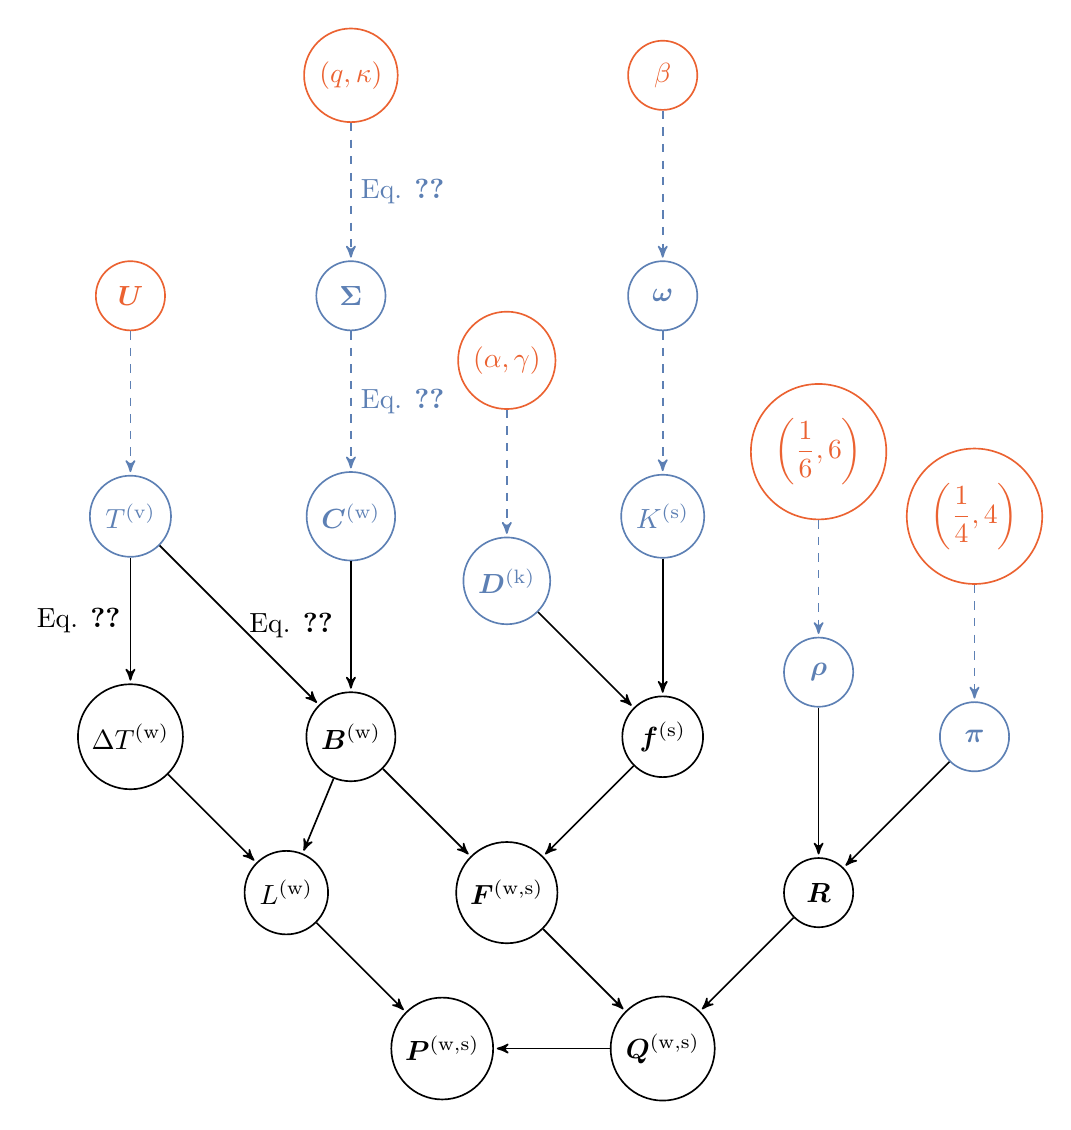
\begin{tikzpicture}[->,>=stealth',shorten >=1pt,auto,node distance=2.8cm,semithick]
	\tikzstyle{every state}=[]
	
	\node[state] (P)                              {$\Probmatrix\branchsiteexp$};
	\node[state] (Q)     [right of=P]             {$\Submatrix\branchsiteexp$};
	\node[state] (L)     [above left of=P]        {$\branchlength\branchexp$};
	\node[state] (F)     [above left of=Q]        {$\ScaledFit\branchsiteexp$};
	\node[state] (R)     [above right of=Q]       {$\Mutmatrix$};
	\node[state] (dT)    [above left of=L]        {$\branchtime\branchexp $};
	\node[state] (Bb)    [above left of=F]        {$\brownian\branchexp $};
	\node[state] (f)     [above right of=F]       {$\Fit\siteexp $};
	\node[state] (Ex)    [BLUE, above of=R]       {$\Exchan$};
	\node[state] (Equi)  [BLUE, above right of=R] {$\Mutequi$};
	\node[state] (T)     [BLUE, above of=dT]      {$\age\nodeexp$};
	\node[state] (C)     [BLUE, above of=Bb]      {$\contrast\branchexp$};
	\node[state] (Base)  [BLUE, above left of=f]  {$\Base\catexp$};
	\node[state] (cat)   [BLUE, above of=f]       {$\catvar\siteexp$};
	\node[state] (ExH)   [RED, above of=Ex]            {$\left( \dfrac{1}{6}, 6\right)$};
	\node[state] (EquiH) [RED, above of=Equi]          {$\left( \dfrac{1}{4}, 4\right)$};
	\node[state] (Unif)  [RED, above of=T]      {$\uniform$};
	\node[state] (Cov)   [BLUE, above of=C]       {$\covariance$};
	\node[state] (baseH) [RED, above of=Base]          {$\left(\baseconc, \Basecenter \right)$};
	\node[state] (sb)    [BLUE, above of=cat]     {$\StickBreaking$};
	\node[state] (CovH)  [RED, above of=Cov]           {$\left(\covariancedf, \covariancekappa\right)$};
	\node[state] (sbH)   [RED, above of=sb]            {$\stickbreakinghyper$};
	
	\path 
	(Q)      edge                node {} (P)
	(L)      edge                node {} (P)
	(F)      edge                node {} (Q)
	(R)      edge                node {} (Q)
	(dT)     edge                node {} (L)
	(Bb)     edge                node {} (L)
	         edge                node {} (F)
	(f)      edge                node {} (F)
	(Ex)     edge                node {} (R)
	(Equi)   edge                node {} (R)
	(T)      edge                node [left]{Eq. \ref{eq:ageTobranchtime}} (dT)
	         edge                node [right]{Eq. \ref{eq:independent_contrast}} (Bb)
	(C)      edge                node {} (Bb)
	(Base)   edge                node {} (f)
	(cat)    edge                node {} (f)
	(ExH)    edge [BLUE, dashed] node {} (Ex)
	(EquiH)  edge [BLUE, dashed] node {} (Equi)
	(Unif)   edge [BLUE, dashed] node {} (T)
	(Cov)    edge [BLUE, dashed] node [right]{Eq. \ref{eq:Distribcontrast}} (C)
	(baseH)  edge [BLUE, dashed] node {} (Base)
	(sb)     edge [BLUE, dashed] node {} (cat)
	(CovH)   edge [BLUE, dashed] node [right]{Eq. \ref{eq:Distribcovariance}} (Cov)
	(sbH)    edge [BLUE, dashed] node {} (sb);
	\end{tikzpicture}
	\caption{\textbf{Directed acyclic graph of dependencies between variables}. Nodes of the directed acyclic graph are the variables, and edges are the functions. Hyper-parameters are depicted in {\color{RED}{red}} circle, random variables in {\color{BLUE}{blue}} circles, and transformed variables in black. Dotted {\color{BLUE}{blue}} line denotes a drawing from a random distribution, and black solid lines denotes a function. }
\end{figure}

\subsection{Model assumptions}

The model defined above makes the following explicit and implicit assumptions:
\begin{itemize}
	\setlength\itemsep{-0.25em}
	\item Known species tree and gene tree, meaning no paralogs and/or horizontal transfers.
	\item No epistasis, meaning independence between sites.
	\item Each sites is assigned a fitness profile, meaning different site of the sequence can share the same fitness profile.
	\item Inside each fitness profile, the fitness of each amino-acids is estimated.
	\item $\Ne$ and $u$ are correlated Brownian processes, giving each branch of the tree different $\Ne$ and $u$ estimates.
\end{itemize}

The input data is an alignment of $ 3 \times \Nsite \times \Ntaxa $ nucleotides and a rooted tree of $2 \times \Ntaxa - 2 $ branches.

\subsubsection{Dated tree}

The topology of the rooted phylogenetic tree is supposed to be known and is not estimated by the model. 
The model estimates the dates at which branches split, thus the dated tree requires $\Ntaxa - 2$ internal node ages that are free parameters. 
Once the node ages ($\age^{(\node)}$) are defined, the time of the branch is defined as the difference in ages between the two edges of the branch:
\begin{equation}
\label{eq:ageTobranchtime}
\branchtime \branchexp =  \age^{(\up)} - \age^{(\down)} 
\end{equation}
By definition, leaf ages are all set to $0$. The root age is set arbitrarily to $1$, but if fossils data are also available the dated tree can be re-scaled into absolute time using cross-multiplication.

\subsubsection{Brownian process $\Ne$ and $\mu$}

The mutation rate per unit of time ($\mu$) and the effective population size ($\Ne$) are assumed to evolve continuously along the phylogeny. Theses fluctuations are modeled by a multivariate Brownian process at each node of tree ($\node$), including the root and the leaves. We assume a logarithm transformation between the Brownian process and our variable $\mu$ and $\Ne$.
\begin{equation}
\brownian^{(\node)}=\left(\ln\left(\Ne^{(\node)}\right), \ln\left(\mu^{(\node)}\right)\right)
\end{equation}
The rate of change of the Brownian process per unit of time is constant and determined by the covariance matrix $\covariance$.
\begin{equation}
\covariance = \begin{pmatrix}
\sigma_{\Ne}^2 & \sigma_{\Ne, \mu}  \\ 
\sigma_{\Ne, \mu} & \sigma_{\mu}^2 \\ 
\end{pmatrix},
\end{equation}
Along a branch ($\branch$) of the tree, the Brownian process starts at the upper node ($\up$), and ends at the supporting youngest node of the branch ($\down$). The process ran during $\branchtime\branchexp$ unit of time, and thus the distribution of $\brownian^{(\up)}$ is:
\begin{equation}
\brownian^{(\up)} - \brownian^{(\down)}  \sim \mathcal{N}\left(\bm{0}, \covariance \branchtime\branchexp \right)
\end{equation}
We make a change of variable as to define the branch-wise independent contrast $\contrast\branchexp$:
\begin{equation}
\label{eq:independent_contrast}
\contrast\branchexp = \dfrac{\brownian^{(\up)} - \brownian^{(\down)}}{\branchtime\branchexp} 
\end{equation}
And these contrasts are i.i.d. from a multivariate normal distribution:
\begin{align}
\label{eq:Distribcontrast}
\contrast\branchexp & \sim \mathcal{N}\left(\bm{0}, \covariance \right) \\
\Rightarrow \ln \left(p_{\contrast\branchexp}\left(\bm{x}\right)\right) & = - \dfrac{1}{2}\left[\ln \left( 4\pi^2 \left| \covariance \right| \right) + \bm{x}^{\mathrm{T}} \covariance^{-1} \bm{x} \right]
\end{align}
The values of the Brownian process are obtained at the $2$ boundary nodes ($\up$ and $\down$) of the branch. However we are interested into the average over the branch to define the codon substitution matrices. In the case of Brownian process, the most likely path (or geodesic) from $\brownian^{(\up)}$ at time $T^{(\up)}$ to $\brownian^{(\down)}$ at time $T^{(\down)}$ is the straight line, and therefore, it would make sense to take the mean value of $\e^{\brownian^{(\node)}}$ along this geodesic, which is equal to:
\begin{equation}
\left(\Ne\branchexp, \mu\branchexp\right) = \dfrac{\e^{\brownian^{(\up)}} - \e^{\brownian^{(\down)}}}{\brownian^{(\up)} - \brownian^{(\down)}}
\end{equation}
Where in the limiting case of $\brownian^{(\up)}$ tending to $\brownian^{(\down)}$, the geodesic tends to:
\begin{equation}
\lim_{\brownian^{(\up)} \to \brownian^{(\down)}} \left(\Ne\branchexp, \mu\branchexp\right) =  \e^{\brownian^{(\down)}}
\end{equation}
The prior on the precision matrix is an invert Wishart distribution, parameterized by $\covariancekappa=1$ and with $\covariancedf=3$ degrees of freedom:
\begin{align}
\label{eq:Distribcovariance}
\covariance & \sim \mathrm{Wishart}^{-1} (\covariancekappa \bm{I}, \covariancedf)
\end{align}
The $2$-dimensional Brownian process requires $ 2 \times \Nnode =  4 \times \Ntaxa - 2 $ parameters.
$\Ne$ at the root is set to $1.0$ for identifiability of the fitness profiles, leaving $4 \times \Ntaxa - 3 $ free parameters.
The $2$-dimensional precision matrix of the Brownian process requires $2 \times (2 + 1) / 2 = 3$ parameters, since the matrix is symmetric.
The $2$-dimensional precision matrix requires $2$ hyper-parameters, fixed to $\covariancekappa=1.0$ and $df=3$.

\subsubsection{Branch length}

The length of a branch is the expected number of substitution per site we should observe along this branch if the process is at equilibrium and under no selection. In first approximation, the branch length multiplied by the number of coding site can the seen as the number of substitutions we would expect to see on the third codon position along this branch.
Formally, the branch length is the product of time ($\branchtime\branchexp$) and mutation rate ($\mu\branchexp$ per unit of time). 
\begin{align}
\branchlength \branchexp & = \mu\branchexp \branchtime\branchexp \nonumber \\
			  & = \mu\branchexp \left( T^{(\up)} - T^{(\down)} \right)
\end{align}


\subsubsection{Nucleotide rate matrix}

The generalized time-reversible nucleotide mutation rate matrix $\Mutmatrix$ is a function of the nucleotide frequencies $\Mutequi$ and the relative rate $\Exchan$. $\Mutequi = (\mutequi_A , \mutequi_C , \mutequi_G , \mutequi_T)$ is the equilibrium base frequency vector, giving the frequency at which each base occurs at each site. $\Exchan = \left( \exchan_{AC}, \exchan_{AG}, \exchan_{AT}, \exchan_{CG}, \exchan_{CT}, \exchan_{GT}\right)$ is the vector of exchangeabilities between nucleotides. Altogether, the rate matrix is:
\begin{equation}
\Mutmatrix = \begin{pmatrix}
- & {\exchan_{AC} \mutequi_C} & {\exchan_{AG}\mutequi_G} & {\exchan_{AT}\mutequi_T} \\ 
{\exchan_{AC}\mutequi_A} & - & {\exchan_{CG}\mutequi_G} & {\exchan_{CT}\mutequi_T} \\ 
{\exchan_{AG}\mutequi_A} & {\exchan_{CG}\mutequi_C} & - & {\exchan_{GT}\mutequi_T} \\  
{\exchan_{AT}\mutequi_A} & {\exchan_{CT}\mutequi_C} & {\exchan_{GT}\mutequi_G} & - 
\end{pmatrix},
\end{equation}
By definition, the sum of the entries in each rows of the nucleotide rate matrix $\Mutmatrix$ is equal to $0$, giving the diagonal entries:
\begin{equation}
\mutmatrix_{a,a} = \sum_{ b \neq a, b \in \SetNuc} \mutmatrix_{a,b}
\end{equation}
The prior on the exchangeabilities $\Exchan$ is an uniform Dirichlet distribution of dimension $6$:
\begin{align}
\Exchan & \sim \mathrm{Dir}\left( \left( \dfrac{1}{6}, \hdots , \dfrac{1}{6} \right) , 6\right) \\
\Rightarrow \ln \left(p_{\Exchan}\left(\bm{x}\right)\right) & = \ln \left(\Gamma(6)\right) - 6\ln\left(\Gamma(1)\right), 
\end{align}
where, 
\begin{equation}
\Gamma(z) = \int_{0}^{\infty} x^{z-1} \e^{-x} \der x.
\end{equation}
Moreover, the equilibrium base frequencies $\Mutequi$ are also normalized to sum to $1$: 
\begin{equation}
\sum_{a \in \SetNuc} \mutequi_a  = 1
\end{equation}
The prior on the equilibrium base frequencies $\Mutequi$ is an uniform Dirichlet distribution of dimension $4$:
\begin{align}
\Mutequi & \sim \mathrm{Dir}\left( \left( \dfrac{1}{4}, \hdots , \dfrac{1}{4} \right) , 4\right) \\
\Rightarrow \ln \left(p_{\Mutequi}\left(\bm{x}\right)\right) & = \ln \left(\Gamma(4)\right) - 4\ln\left(\Gamma(1)\right), 
\end{align}

The general time-reversible nucleotide matrix requires $5+3 = 8$ free parameters. Moreover, the matrix is normalized such that we expect $1$ substitution per unit of branch length. Thus we can find the expected rate of change by calculating the sum of flux out of each state weighted by the proportion of sites that are expected to be in that class:
\begin{equation}
\sum_{a \in \SetNuc} - \mutequi_a \mutmatrix_{a,a} = 1.
\end{equation}
The generalized time-reversible nucleotide rate matrix thus requires $7$ free parameters after normalization.

\subsubsection{Fitness profiles}

Each sites is assigned to a fitness profile, requiring $\Nsite$ free parameters.
The fitness profiles require $20 \times \text{N}_{\text{category}} $ parameters, one fitness for each amino-acid.
Since only the difference in fitness matters, for identifiability, one of the fitness for each profile can arbitrarily be set to $0.0$, leaving $19 \times \text{N}_{\text{category}} $ free parameters.
$???$ hyper-parameters are required for the fitness profiles.

\begin{align}
\ScaledFit\catexp & \sim \mathrm{Dir}\left( \left( \dfrac{1}{20}, \hdots , \dfrac{1}{20} \right) , 20\right) \\
\Rightarrow \ln \left(p_{\Mutequi}\left(\bm{x}\right)\right) & = \ln \left(\Gamma(20)\right) - 20\ln\left(\Gamma(1)\right), 
\end{align}


\subsubsection{Codon substitution rates and equilibrium frequencies}

For a given branch $\branch$ and a given site $\site$, the codon substitution rate matrix $\Submatrix\branchsiteexp$ is given by:
\begin{equation}
\begin{dcases}
 \submatrix\branchsiteexp_{\itoj} = 0\text{ if } \cj \notin \Ni \text{ and } \ci \neq \cj, \\
 \submatrix\branchsiteexp_{\itoj} = \mu\branchexp \mutmatrix_{\nucitoj}\text{ if } \cj \in \NiSyn, \\
 \submatrix\branchsiteexp_{\itoj} = \mu\branchexp \mutmatrix_{\nucitoj} \dfrac{4\Ne\branchexp \left({\fitj\catsiteexp - \fiti\catsiteexp}\right)}{{1 - \e^{4\Ne\branchexp\left({\fiti\catsiteexp - \fitj\catsiteexp}\right)} }}\text{ if } \cj \in \NiNonSyn,\\
 \submatrix\branchsiteexp_{\ci, \ci} = - \sum_{ \cj \neq \itoj \in \SetCodon} \submatrix\branchsiteexp_{\itoj}
\end{dcases}
\end{equation}
And the codon equilibrium frequencies $\Subequi$ are given by
\begin{equation}
\subequi_{\ci}\branchsiteexp = \mutequi_{\ci_1} \mutequi_{\ci_2} \mutequi_{\ci_3} \e^{4 \Ne\branchexp \fiti\catsiteexp}
\end{equation}
For each branch and site, we have the reversibility of the substitution process:
\begin{equation}
\subequi_{\ci}\branchsiteexp \submatrix\branchsiteexp_{\itoj} = \subequi_{\cj}\branchsiteexp \submatrix\branchsiteexp_{\cj, \ci}
\end{equation}
And for the root, $\Ne$ is set to $1$ for identifiability of the substitution process:
\begin{equation}
\subequi_{\ci}^{\rootsiteexp} = \mutequi_{\ci_1} \mutequi_{\ci_2} \mutequi_{\ci_3} \e^{4 \fiti\catsiteexp} 
\end{equation}
\begin{figure}[H]
	\centering
	\includegraphics[width=\textwidth]{Artworks/nodemutsel.jpg}
\end{figure}

\subsection{Likelihood of divergence data}
\begin{itemize}
	\item $\tau$ is the tree with given branch lengths ($d_i$).
	\item $\mu$ is mutation matrix ($4\mathrm{x}4$).
	\item $\ScaledFit^{k}$ is the fitness vector ($1\mathrm{x}20$) of amino-acids at site $k$.
	\item $\Data=\{\si, \sii, \siii, \siiii \}$ is the observed data at the leaves, at site $k$.
	\item $\s$ and $\siiiii$ are the unknown states of the internal nodes, at site $k$.
	\item $\pi(\s)$ is the equilibrium frequency of state $\s$.
\end{itemize}
Likelihood of the data at site $k$, given all possible states of internal node is:
\begin{equation*}
P\left(\Data| \tau, \mu, \ScaledFit^{k}\right) = \sum_{\s=1}^{61}  \sum_{\siiiii=1}^{61} \pi(\s) \cdot P_{\s \si}(d_1) \cdot P_{\s \sii}(d_2) \cdot P_{\s \siiiii}(d_5) \cdot P_{\siiiii \siii}(d_3) \cdot P_{\siiiii \siiii}(d_4) 
\end{equation*}
For an inner node $i$ with offspring $o_1$ and $o_2$, $L_{i} \left( \sn, \tau, \mu, \ScaledFit^{k} \right)$ is defined recursively as:
\begin{equation*}
L_{i} \left( \sn, \tau, \mu, \ScaledFit^{k} \right) = \left[ \sum_{x=1}^{61} P_{\sn x }(d_{o_1}) L_{o_1}\left( x, \tau, \mu, \ScaledFit^{k} \right) \right] \cdot \left[ \sum_{x=1}^{61} P_{\sn x }(d_{o_2}) L_{o_2}\left( x, \tau, \mu, \ScaledFit^{k} \right) \right]
\end{equation*}
And for a leaf $i$:
\begin{equation*}
L_{i}\left( \sn, \tau, \mu, \ScaledFit^{k}\right) =
\begin{dcases}
1, & \text{if } \sn = {\color{PINK}{\scaledselcoef_i^{k}}} \\
0, & \text{otherwise.}
\end{dcases}
\end{equation*}
Then the likelihood of the data at site $k$, given all possible states of internal node is:
\begin{equation*}
P\left(\Data| \tau, \mu, \ScaledFit^{k}\right) = \sum_{x=1}^{61} \pi(x) L_{\text{root}} \left( x | \tau, \mu, \ScaledFit^{k} \right)
\end{equation*}

\subsection{Substitution mapping, sufficient statistics, and partial-likelihood}

\subsubsection{Scatter sufficient statistics}

From the independent contrast $\contrast\branchexp$ (equation~\ref{eq:independent_contrast}) of the Brownian process $\brownian^{(\node)}$, we can define the $2 \times 2$  scatter sufficient statistic matrix, $\bm{A}$ as:
\begin{equation}
\bm{A} = \sum_{b=1}^{\Nbranch} \contrast\branchexp. \left[\contrast\branchexp\right]^{\mathrm{T}}
\end{equation}
By Bayes theorem, the posterior on $\Sigma$, conditional on a particular realization of $\brownian$ (and thus of $\contrast$) is an invert Wishart distribution, of parameter $\covariancekappa \bm{I} + \bm{A}$ and with $\Nbranch + 3$ degrees of freedom.
\begin{equation}
\covariance | \brownian, \Nbranch, \covariancekappa  \sim \mathrm{Wishart}^{-1}\left( \covariancekappa \bm{I} + \bm{A}, \Nbranch + 3\right)
\end{equation}
This invert Wishart distribution can be obtained by sampling $\Nbranch + 3$ independent and identically distributed multivariate normal random variables $\bm{Z}_{k}$ defined by
\begin{equation}
\bm{Z}_{k} \sim \mathcal{N} \left( \bm{0}, \left[\covariancekappa \bm{I} + \bm{A}\right]^{-1} \right).
\end{equation}
And from these multivariate samples, $\covariance$ is Gibbs sampled as:
\begin{equation}
\covariance = \left( \sum_{k=1}^{\Nbranch + 3} \bm{Z}_{k}.\bm{Z}_{k}^{\mathrm{T}} \right)^{-1}
\end{equation}

\subsubsection{Substitution mapping}

A sequence of length $\Nsite$ evolves by point substitutions, according to a random process defined by the substitutions matrices $\Submatrix\branchsiteexp$, over a phylogenetic tree.
A realization of the random process results in a detailed substitution history over the tree, which will be denoted by $\history$.
The substitution history at branch $\branch$ and site $\site$ will be denoted by $\history\branchsiteexp$.

\subsubsection{Path sufficient statistics}

If we express the probability of the substitution mapping ($\history\branchcatexp$) as a function of the codon substitution process, we get the following expression:
\begin{equation}
\label{eq:PathSuffStat}
p(\history\branchcatexp | \branchlength\branchexp, \Submatrix\branchcatexp) \propto \prod_{\ci \in \SetCodon} \left[\subequi_{\ci}\branchcatexp\right]^{n_{\ci}\branchcatexp} \prod_{ \left(\ci, \cj\right) \in \SetCodon^2} \left[\submatrix\branchcatexp_{\itoj}\right]^{m_{\ci, \cj}\branchcatexp} \prod_{\ci \in \SetCodon} \e^{- \left|  \submatrix\branchcatexp_{\ci, \ci}\right| a_{\ci}\branchcatexp}
\end{equation}
where we define the sufficient statistics:
\begin{itemize}
	\setlength\itemsep{-0.25em}
	\item $m_{\ci, \cj}\branchcatexp$ is the total number of substitutions from codon $\ci$ to codon $\cj$
	\item $n_{\ci}\branchcatexp$ is the number of sites starting with codon $\ci$ at the tip of the branch.
	\item $a_{\ci}\branchcatexp$ is the total waiting time in codon $\ci$.
\end{itemize}
Once these sufficient statistics have been computed, the parameters of the substitution matrix $\Submatrix\branchcatexp$ can be resampled conditional on $\history\branchcatexp$, 
using equation~\ref{eq:PathSuffStat} each time the likelihood needs to be recomputed. This leads to relatively fast MCMC strategy.

\subsubsection{Length sufficient statistics}

In the case of branch lengths, sufficient statistics take a very simple form:
\begin{equation}
\label{eq:LengthSuffStat}
p(\history\branchexp | L\branchexp) \propto \prod_{\ci \in \SetCodon} \left[ l_{\ci}\branchexp\right]^{u_{\ci}\branchexp} \e^{- b_{\ci}\branchexp L_{\ci}\branchexp}
\end{equation}
where we define the sufficient statistics:
\begin{itemize}
	\setlength\itemsep{-0.25em}
	\item $u_{\ci}\branchexp$ is the total number of substitutions over branch $\branch$, summed over all sites.
	\item $b_{\ci}\branchexp$ is the mean rate away from current codon state (averaged over the entire substitution history).
\end{itemize}
Thus, formally, the probability of the substitution mapping can be summarized by saying that the total number of substitutions along a given branch over all sites, $u_{\ci}$, is Poisson distributed, of mean $b_{\ci} l_{\ci}$.


\section{Inferring demography with divergence and polymorphism data}

Less sensitive to assumption of no epistasis and static fitness landscape.
The first strategy is to augment information about interspecies conservation with information about genetic polymorphism.

\subsection{Model assumptions and definition}

\subsubsection{Assumptions}

\begin{itemize}
	\setlength\itemsep{-0.25em}
	\item Known species tree and gene tree, meaning no paralogs and/or horizontal transfers.
	\item No epistasis, meaning independence between sites.
	\item Each sites is assigned a fitness profile, meaning different site of the sequence can share the same fitness profile.
	\item Inside each fitness profile, the fitness of each amino-acids is estimated.
	\item $\Ne$, $u$ and $\tau$ are correlated Brownian processes, giving each branch of the tree different $\Ne$, $u$ and $\tau$ estimates.
\end{itemize}

\subsubsection{Wright-Fisher process for a single site}

The Wright-Fisher process describe the change in frequency of single polymorphic site with two alleles in a population over time.
The model makes the following assumptions:
\begin{itemize}
	\setlength\itemsep{-0.2em}
	\item Non-overlapping generations
	\item Constant population size in each generation
	\item Random mating
\end{itemize}
Consider a population of $\Ne$ diploid individuals that has a single polymorphic site with two alleles, one ancestral (fitness = $1$) and one derived (fitness = $1+\selcoef$).
Assuming no dominance and no recurrent mutation, the probability, that there are $j$ copies of the derived allele present at generation $G+1$ (denoted $X_{G+1}$) given i copies of the derived allele present at generation $G$ (denoted $X_{G}$) is given by the following binomial calculation:
\begin{equation}
	p\left( X_{G+1} = j |X_{G} = i, \Ne, \selcoef \right)  =  \binom{2 \Ne}{j} \left( \dfrac{x(1+\selcoef)}{x(1+\selcoef) + (1-x)} \right)^j \left(1 - \dfrac{x(1+\selcoef)}{x(1+\selcoef) + (1-x)} \right)^{2 \Ne -j}, 
\end{equation}
where $x = i / 2 \Ne$ is the derived allele frequency in generation $G$.\\

In this discrete framework, it has been shown to be extremely difficult to explicitly derive formulas for several quantities of evolutionary interest.
However, as the size of the population approaches infinity (i.e.
$ \Ne \rightarrow \infty$), and assuming that the scaled selection pressure ($\Ne \selcoef $) remain constant, the discrete Markov process given above can be closely approximated by a continuous-time, continuous-space diffusion process.\\

Under the assumption of no recurrent mutation, the derived allele with initial frequency $p$, goes either extinct ($x=0$) or fixed ($x=1$) after a long time.
It is possible to determine the probability of fixation ($p_{\mathrm{fix}}$), by using the Kolmogorov backward equation.
\begin{equation}
	p_{\mathrm{fix}}(p, \scaledselcoef ) = \dfrac{1 - \e^{-\scaledselcoef p }}{1 - \e^{-\scaledselcoef}}\text{, where } \scaledselcoef=4\Ne \selcoef 
\end{equation}
\begin{figure}[H]
	\centering
	\begin{tikzpicture}
	\begin{axis}[
	ylabel={$p_{\mathrm{fix}}(p, \scaledselcoef )$},
	xlabel={Initial population frequency ($p$)},
	domain=0:1,
	cycle list name=colors,
	samples=100,
	legend entries={$\scaledselcoef=12$, $ \scaledselcoef=4$, $\scaledselcoef=0$, $\scaledselcoef=-4$, $\scaledselcoef=-12$},
	legend cell align=left,
	minor tick num=2,
	axis x line=bottom,
	axis y line=left,
	legend style={at={(0.1,0.9)},anchor=north west}
	]
	\addplot{(1 - exp(-12 * x)) / (1 - exp(- 12))};
	\addplot{(1 - exp(-4 * x)) / (1 - exp(- 4))};
	\addplot{x};
	\addplot{(1 - exp(4 * x)) / (1 - exp(4))};
	\addplot{(1 - exp(12 * x)) / (1 - exp(12))};
	\end{axis}
	\end{tikzpicture}
	\caption{\textbf{}}
\end{figure}
$g(x, \scaledselcoef) \der x $ is the expected time for which the population frequency of the derived allele, at the site, is in the range $(x, x+\der x)$ before eventual absorption:
\begin{align}
	g(x, \scaledselcoef) & \approx  \dfrac{2 \left[ 1 - \e^{-\scaledselcoef (1-x)}\right]}{(1 - \e^{-\scaledselcoef})x(1-x)}
\end{align}
\begin{figure}[H]
	\centering
	\begin{tikzpicture}
	\begin{axis}[
	ylabel={$g(x, \scaledselcoef)$},
	xlabel={frequency of the derived allele ($x$)},
	domain=0.05:0.95,
	cycle list name=colors,
	samples=100,
	legend entries={$\scaledselcoef=12$, $ \scaledselcoef=4$, $\scaledselcoef=0$, $\scaledselcoef=-4$, $\scaledselcoef=-12$},
	legend cell align=left,
	minor tick num=2,
	axis x line=bottom,
	axis y line=left,
	legend style={at={(0.1,0.9)},anchor=north west}
	]
	\addplot{2 * (1 - exp(-12 * (1-x))) / ((1 - exp(-12))*x*(1-x))};
	\addplot{2 * (1 - exp(-4 * (1-x))) / ((1 - exp(-4))*x*(1-x))};
	\addplot{2 / x};
	\addplot{2 * (1 - exp(4 * (1-x))) / ((1 - exp(4))*x*(1-x))};
	\addplot{2 * (1 - exp(12 * (1-x))) / ((1 - exp(12))*x*(1-x))};
	\end{axis}
	\end{tikzpicture}
	\caption{\textbf{}}
\end{figure}

\subsubsection{Poisson random fields in Mutation-Selection framework }

S. Sawyer and D. Hartl expanded the modeling of site evolution to multiple sites.
The model makes the following assumptions: 
\begin{itemize}
	\setlength\itemsep{-0.2em}
	\item Mutations arise at Poisson times (rate $u$ per site per generation)
	\item Each mutation occurs at a new site (infinite sites, irreversible)
	\item Each mutant follows an independent Wright-Fisher process (no linkage)
\end{itemize}
In a sample of size $\samples$, the expected number of sites with $k$ (which ranges from $1$ to $\samples-1$) copies of the derived allele is defined as a function of $g(x)$:
\begin{align}
	G(\copies, \samples, \theta, \scaledselcoef) & = 2 \Ne u \int_{0}^{1} g(x, \scaledselcoef)  \binom{\samples}{\copies} x^{\copies} (1-x)^{\samples-\copies} \der x \nonumber \\
	& = \theta \int_{0}^{1} \dfrac{1 - \e^{-\scaledselcoef (1-x)}}{(1 - \e^{-\scaledselcoef})x(1-x)} \binom{\samples}{\copies} x^{\copies} (1-x)^{\samples-\copies} \der x\text{, where } \theta=4\Ne u \nonumber \\
	& = \binom{\samples}{\copies} \dfrac{\theta }{1 - \e^{-\scaledselcoef}} \int_{0}^{1} \left( 1 - \e^{-\scaledselcoef (1-x)} \right) x^{\copies-1} (1-x)^{\samples-\copies-1} \der x
\end{align}
In the mutation selection-framework developed, the fitness of a given genotype is a function of the encoded amino-acid through the site-wise amino-acid fitness profiles ($ \Fit\siteexp $ at site $\site$). Thus the coefficient ($\scaledselcoef=4\Ne \selcoef $) associated to a mutation is a function of the amino-acids encoded by the ancestral ($\ci$) and derived ($\cj$) codon. Altogether the selection coefficient from $\ci$ to $\cj$ at site $\site$ is:
\begin{align}
\scaledselcoef_{\itoj}(\Ne, \Fit\siteexp) &= 4 \Ne (f_\cj\siteexp-f_\ci\siteexp) \nonumber \\
& = \scaledfit_\cj\siteexp-\scaledfit_\ci\siteexp
\end{align}
Similarly, the mutation rate between by the ancestral ($\ci$) and derived ($\cj$) codon is a function of the nucleotide changes between the codons. If the codons are not neighbor, meaning a single mutation is not sufficient to jump from $\ci$) to $\cj$, the mutation rate is equal to $0$. If the codons are neighbors, the mutation rate is given by the nucleotide rate matrix ($ \bm{u} $). Altogether, the scaled mutation rate $\theta_{\itoj}$ from $\ci$ to $\cj$ is:
\begin{equation}
\theta_{\itoj}(\Ne, u, \Mutmatrix) = 4 \Ne u \mutmatrix_{\itoj}
\end{equation}
If a site is polymorphic and the ancestral ($\ci$) and derived ($\cj$) codons are neighbors, the probability of observing $\copies$ copies ($\samples \geq \copies > 0$) of the derived codon ($\cj$), in a sample of size $\samples$, at site $\site$, is given by:
\begin{equation}
  P(\ci=\samples-\copies,\cj=\copies \ |\ \Ne, u, \Mutmatrix, \Fit\siteexp)  =  G\left(\copies, \samples, \theta_{\itoj}(\Ne, u, \Mutmatrix), \scaledselcoef_{\itoj}(\Ne, \Fit\siteexp) \right)
\end{equation}
Moreover the probability that a site is monomorphic is given by:
\begin{equation}
 P(\ci= \samples \ |\ \Ne, u, \Mutmatrix, \Fit\siteexp)  = 1 - \sum_{\cj \in \Ni} \sum_{\copies=1}^{\samples}  G\left(\copies, \samples, \theta_{\itoj}(\Ne, u, \Mutmatrix),  \scaledselcoef_{\itoj}(\Ne, \Fit\siteexp)\right)
\end{equation}
And all other probabilities equal to $0.0$.

\subsection{Substitution mapping, sufficient statistics, and partial-likelihood}

\subsubsection{Pruning and substitution mapping}

\subsubsection{Polymorphism sufficient statistics}

\subsection{$\Ne$, $u$ and $\tau$ inference in BayesCode}
    
    
\end{document}
